\part{Exercice 5}

\begin{enumerate}
	\item On a \[
			\overline{A} = \{f\}^n \cup \{g\}^n
		\] donc
		\begin{align*}
			P(A) &= 1 - P(\overline{A}) \\
			&= 1 - \frac{2}{2^n} \\
			&= \frac{2^n - 2}{2^n}. \\
		\end{align*}
		Et, \[
			B = \{g\}^n \cup \{(f,g,\ldots,g)\} \cup \{(g,f,g,\ldots,g)\} \cup \cdots \cup \{(g, \ldots, g, f)\}
		\] donc $P(B) = \frac{n+1}{2^n}$.
	\item $P(A \cap B) = \frac{n}{2^n}$ et $P(A)\,P(B) = \frac{2^n-2}{2} \times \frac{n+1}{2^n}$ d'où
		\begin{align*}
			&P(A \cap B) = P(A)\,P(B)\\
			\iff& n 2^n = (2^n - 2)(n+1)\\
			\iff& 2^n - 2n - 2 = 0\\
			\iff& 2^{n-1} - n - 1 = 0?
		\end{align*}

		Soit $f : x\mapsto 2^{x-1} - x - 1$ dérivable sur $\R$ et \[
			\forall x \in \R,\,f'(x) = \ln(2) 2^{x-1} - 1
		.\] Soit $x \in \R$.
		\begin{align*}
			f'(x) > 0 \iff& 2^{x-1} > \frac{1}{\ln 2}\\
			\iff& (x-1) \ln 2 > \ln \left( \frac{1}{\ln 2} \right)\\
			\iff& x > \frac{-\ln(\ln 2)}{\ln 2} + 1 \simeq 1,\!5.
		\end{align*}
		Donc, $f$ est strictement croissante sur $[2, +\infty[$.
		\begin{center}
			\begin{tikzpicture}
				\tkzTabInit{$x$/1,$f$/2.3}{$0$, $-\frac{\ln(\ln 2)}{\ln 2}$, $+\infty$}
				\tkzTabVar{+/$<0$, -/{}, +/$+\infty$}
				\tkzTabVal23{0.5}30
			\end{tikzpicture}
		\end{center}

		Donc $n=3$ est la seule solution de $(*)$.
\end{enumerate}

